\section{A Machine Learning Approach to Visual Perception of Forest
Trails for Mobile Robots}\label{header-n5}

\emph{IEEE ROBOTICS AND AUTOMATION LETTERS, VOL. 1, NO. 2, JULY 2016} {[}2{]}

\subsection{Introduction}\label{header-n7}

This article studies the problem of perceiving forest or mountain trails
from a single monocular image acquired from the viewpoint of a robot.
Autonomously following a man-made trail is challenging for robotics.
Many robot types, including wheeled, tracked, and legged vehicles, are
capable of locomotion along real-world trails. Moreover, Micro Aerial
Vehicles (MAVs) flying under the tree are a compelling and realistic
option made possible by recent technological advances. One of the
innovations introduced by this article is that the robot used for the
experiments is a quadrotor: a drone with four rotors. In order to follow
a trail, a robot has to perceive where the trail is, then react in order
to stay on the trail. The robot input is a monocular image from a
forward-looking camera. Perceiving real-world trails in these conditions
is an extremely difficult and interesting pattern recognition problem.
Computer Vision and Robotics literature mainly focused on paved road and
forest/desert road perception. The latter is a significantly more
difficult problem: unpaved roads are normally much less structured than
paved ones. Their appearance is very variable and often boundaries are
not well defined. In addition, their surface appearance can change very
frequently, their shape and width are not as constrained, they often
seamlessly blend with the surrounding area. Previous works deal with the
task of perceiving trails as a segmentation problem, aiming to determine
which areas of the input image corresponding to the image of the trail.
To do this, it is necessary to classify the visual features that
characterize a trail. All of these techniques are conceptually similar
to image saliency. A \emph{saliency map} is an image that shows for each
pixel (of the original image) how much such pixel visually ``stands out"
from the rest. This information, which by itself is expected to be very
noisy, is aggregated in order to infer the trail position and direction
in the image. In this work, the authors follow a different approach and
cast the trail perception problem as an image classification task. The
robot estimates the approximate direction of the trail with respect to
the direction of view by adopting a supervised machine learning approach
based on Deep Neural Networks (DNNs). One of the advantages of DNNs for
supervised image classification is generality: in fact, features are
learned directly from data and do not have to be chosen or modeled by
the algorithm developers for the specific problem. Deep learning is used
also for obstacle avoidance. Previous work shows how imitation learning
can be used to steer a quadrotor to avoid trees in an outdoor
environment. The controller is previously trained by manually piloting
the robot for a short time. However, the visual perception task is
harder, requiring a more powerful classifier to be trained with a
significantly larger training dataset obtained offline.

\subsection{Proposed method}\label{header-n9}

\subsubsection{Problem formulation}\label{header-n10}

The robot consists of a MAV with a monocular camera, fixed in front of
it. The drone flies with a height similar to the average height of a
person (approximately 1.7 meters). The input is an image acquired by the
camera. The main goal is to remain on the trail analyzing the image
using a deep learning module. There are considered three different
classes which correspond to three different actions that the robot
should implement in order to remain on the trail:

\begin{itemize}
\item
  \textbf{Turn Left (TL):} if $−90\degree \textless{} \alpha \textless{} −\beta$; the
  trail is heading towards the left part of the image
\item
  \textbf{Go Straight (GS):} if $−\beta \leq  \alpha \textless{} +\beta$; the trail is
  heading straight ahead, at least in the close range
\item
  \textbf{Turn Right (TR):} if $+\beta \leq \alpha \textless{} +90\degree$; the trail is
  heading towards the right part of the image
\end{itemize}

With $\beta$ = 15\degree.

\begin{figure}[h!]
	\centering
	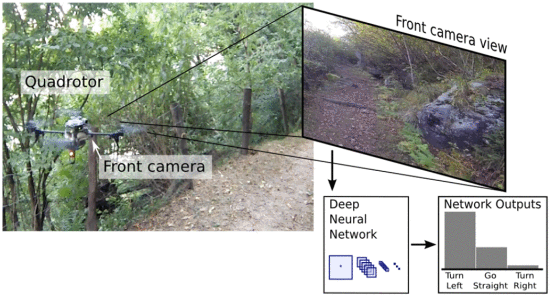
\includegraphics[width=0.8\linewidth]{images/quad.png}
	\caption{The proposed method's overview}
\end{figure}

\subsubsection{Dataset}\label{header-n47}

Recognize a trail is a very hard task and the learning machine needs a
large and well-formed dataset to perform this task effectively. Such a
dataset does not exist and the authors had to create it from scratch. A
hiker was equipped with three head-mounted cameras: one pointing 30◦ to
the left, one pointing straight ahead, and one pointing 30◦ to the
right. The fields of view of the three cameras partially overlap and
cover approximately 180 degrees. The hiker then swiftly walks a long
trail, by taking care of always looking straight along its direction of
motion. The dataset is composed of the images acquired by the three
cameras, labeled as follows: all images acquired by the central camera
are of class GS, those acquired by the right camera are of class TL and
the others (acquired by the left camera) make up the TR class. The
dataset is composed of 8 hours of $1920 \times 1080$ 30fps video acquired using
three GoPro Hero3 Silver cameras and covers approximately 7 kilometers
of hiking trails acquired at altitudes ranging from 300 m to 1200 m,
different times of the day and weather. The dataset has been split into
disjoint training (17,119 frames) and testing (7,355 frames) sets.

\subsubsection{Deep neural network}\label{header-n55}

The authors implement the trail perception module as DNN (deep neural
network), which is a feed-forward network built using successive pairs
of convolutional and max-pooling layers, followed by several fully
connected layers. To improve the network performances, the training set
is augmented by synthesizing left/right mirrored versions of each
training image. Additionally, mild affine distortions ($\pm10\%$
translation, $\pm15^{\circ}$ rotation, $\pm10\%$ scaling) are applied to training
images to further increase the number of samples. The DNN is trained
using backpropagation for 90 epochs, with a learning rate initially set
to 0.005, then scaled by a factor of 0.95 per epoch. The free parameters
(weights) are initialized with random numbers from a uniform
distribution in the range {[}−0.05, 0.05{]} and they are optimized using
stochastic gradient descent. The network has an input layer formed by a
matrix of $3 \times 101 \times 101$ neurons. To fit with the input layer, the images
are first anisotropically resized (with an anti-aliasing technique) to a
size of $101 \times 101$ pixels. The pixels intensity are rescaled to the range
{[}-1, +1{]}. The DNN's output layer has 3 neurons, one for each of the
three classes TL, TR, GS.

\subsubsection{Experimental results}\label{header-n72}

For the three-class classification problem, the absolute accuracy metric
is computed to evaluate the model performances. To have a more robust
performance evaluation, the authors consider a derived two-class
classification problem. The resulting problem consists in determining if
an image is of class GS or not. There are calculated accuracy,
corresponding precision (the proportion of positive classifications that
are actual positives), recall (the proportion of the actual positives
that are identified correctly), and the area under the ROC curve. The
authors compare the DNN performance to three alternatives:

\begin{itemize}
\item
  \textbf{Simple Saliency-based Model:} it is computed a saliency map of
  the input frame, based on the image hue. The saliency map is
  discretized to $16 \times 9$ blocks, and the average saliency for each block
  yields a 144-dimensional feature vector. An SVM model with an RBF
  kernel is learned from the training set to map this feature vector to
  the three-class: TL, GS, and TR.
\item
  \textbf{The method by Santana et al:} this algorithm is explained in
  {[}12{]} and it is applied to the dataset images (50 iterations per
  frame). Its output trail soft segmentation is sampled at each of the
  testing frames.
\item
  \textbf{Two human observers:} each of which is asked to classify 200
  randomly sampled images from the testing set in one of the three
  classes.
\end{itemize}

The obtained results are reported it the following tables.

\begin{longtable}[]{@{}llllll@{}}

\toprule
& \textbf{DNN} & \textbf{Saliency} & \textbf{{[}2{]}} & \textbf{Human1}
& \textbf{Human2}\tabularnewline
\midrule
\endhead
\textbf{Accuracy} & 85.2\% & 52.3\% & 36.5\% & 86.5\% &
82.0\%\tabularnewline
\bottomrule
\caption{Results for the three-class problem}
\end{longtable}

\begin{longtable}[]{@{}llllll@{}}
\toprule
& \textbf{DNN} & \textbf{Saliency} & \textbf{{[}2{]}} & \textbf{Human1}
& \textbf{Human2}\tabularnewline
\midrule
\endhead
\textbf{Accuracy} & 95.0\% & 73.6\% & 57.9\% & 91.0\% &
88.0\%\tabularnewline
\textbf{Precision} & 95.3\% & 60.9\% & 39.8\% & 79.7\% &
84.0\%\tabularnewline
\textbf{Recall} & 88.7\% & 46.6\% & 64.6\% & 95.1\% &
81.6\%\tabularnewline
\textbf{AUC} & 98.7\% & 75.9\% & - & - & -\tabularnewline
\bottomrule
\caption{Results for the two-class problem}
\end{longtable}

\subsubsection{Conclusion}\label{header-n191}

The model has good performance, even when compared to those of humans.
However, problems arise when applying this model in the real world. The
authors implemented this model in a real drone, with a camera that
captures frames with a resolution of $752 \times 480$ pixels. The main problem
is the much lower image quality acquired by the quadrotors' cameras as
compared to the GoPro's images in the training dataset. This yielded a
lower performance of the classifier compared to the testing dataset.
This was especially apparent in situations with strong sky-ground
contrast. Another problem is related to the trail width: the robot is
often unable to negotiate trails if there is not enough free space
beside the trail centerline. Despite this, on wide trails with even
lighting conditions, the robot was able to successfully follow the trail
for a few hundreds of meters.